179. \begin{figure}[ht!]
\center{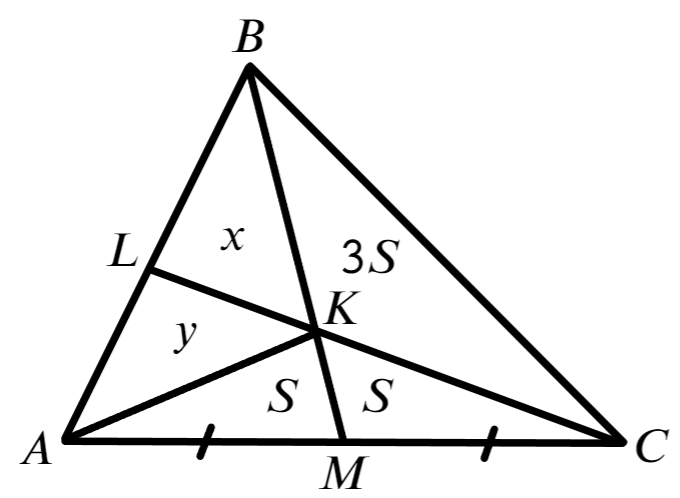
\includegraphics[scale=0.35]{g9-179.png}}
\end{figure}\\
Пусть прямая $CK$ пересекает сторону $AB$ в точке $L.$ Будем пользоваться тем фактом, что площади треугольников с общей высотой относятся так же, как основания, к которым эта высота проведена. Тогда если $S_{\Delta AKM}=S_{\Delta CKM}=S,$ то $S_{\Delta CKB}=3S.$ Пусть $S_{\Delta BKL}=x,\ S_{\Delta AKL}=y.$ Тогда из треугольников $AKL$ с $AKC$ и $BKL$ с $BKC$ получим соотношения $\cfrac{y}{2S}=\cfrac{LK}{CK}=\cfrac{x}{3S},$ откуда $\cfrac{y}{x}=\cfrac{2}{3}.$ Значит, $\cfrac{AL}{LB}=\cfrac{y}{x}=\cfrac{2}{3}.$\\
